\documentclass[border=8pt]{standalone}
\usepackage[utf8]{inputenc}
\usepackage{times}
\usepackage{tikz}
\usetikzlibrary{arrows.meta}

\begin{document}
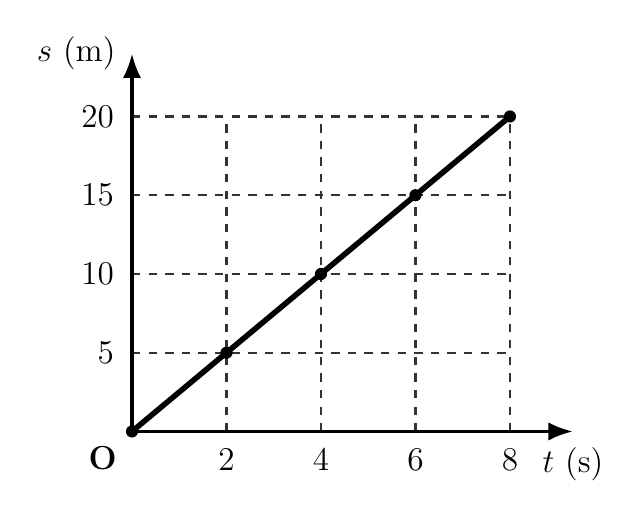
\begin{tikzpicture}[x=1cm, y=1cm, >=Latex, font=\large]
  % Grid
  \draw[dashed, line width=0.75pt, black!80] (0,0) grid[xstep=1.2, ystep=1.0] (4.8,4.0);
  % Axes
  \draw[->, line width=1.3pt] (0,0) -- (5.6,0) node[below=2pt] {$t\mbox{ (s)}$};
  \draw[->, line width=1.3pt] (0,0) -- (0,4.8) node[left=2pt] {$s\mbox{ (m)}$};
  % Ticks & Labels
  \node[below left=2pt] at (0,0) {\textbf{O}};
  \node[below=3pt] at (1.2,0) {2};
  \node[below=3pt] at (2.4,0) {4};
  \node[below=3pt] at (3.6,0) {6};
  \node[below=3pt] at (4.8,0) {8};
  \node[left=3pt] at (0,1.0) {5};
  \node[left=3pt] at (0,2.0) {10};
  \node[left=3pt] at (0,3.0) {15};
  \node[left=3pt] at (0,4.0) {20};
  % Line
  \draw[line width=2.0pt, black] (0,0) -- (4.8,4.0);
  \fill[black] (0,0) circle (2.2pt);
  \fill[black] (1.2,1.0) circle (2.2pt);
  \fill[black] (2.4,2.0) circle (2.2pt);
  \fill[black] (3.6,3.0) circle (2.2pt);
  \fill[black] (4.8,4.0) circle (2.2pt);
\end{tikzpicture}
\end{document}
